\documentclass{article}

\usepackage{graphicx}
\usepackage{tikz}
\usepackage{tikzsymbols}
\usetikzlibrary{calc,patterns,shapes.geometric}
\pagestyle{empty}
\usepackage[margin=0pt]{geometry}
\geometry{papersize={14in,12in}}

\def\centerarc[#1](#2)(#3:#4:#5){\draw[#1] ($(#2)+({#5*cos(#3)},{#5*sin(#3)})$) arc (#3:#4:#5);}

\begin{document}
	\begin{figure}
		\centering
		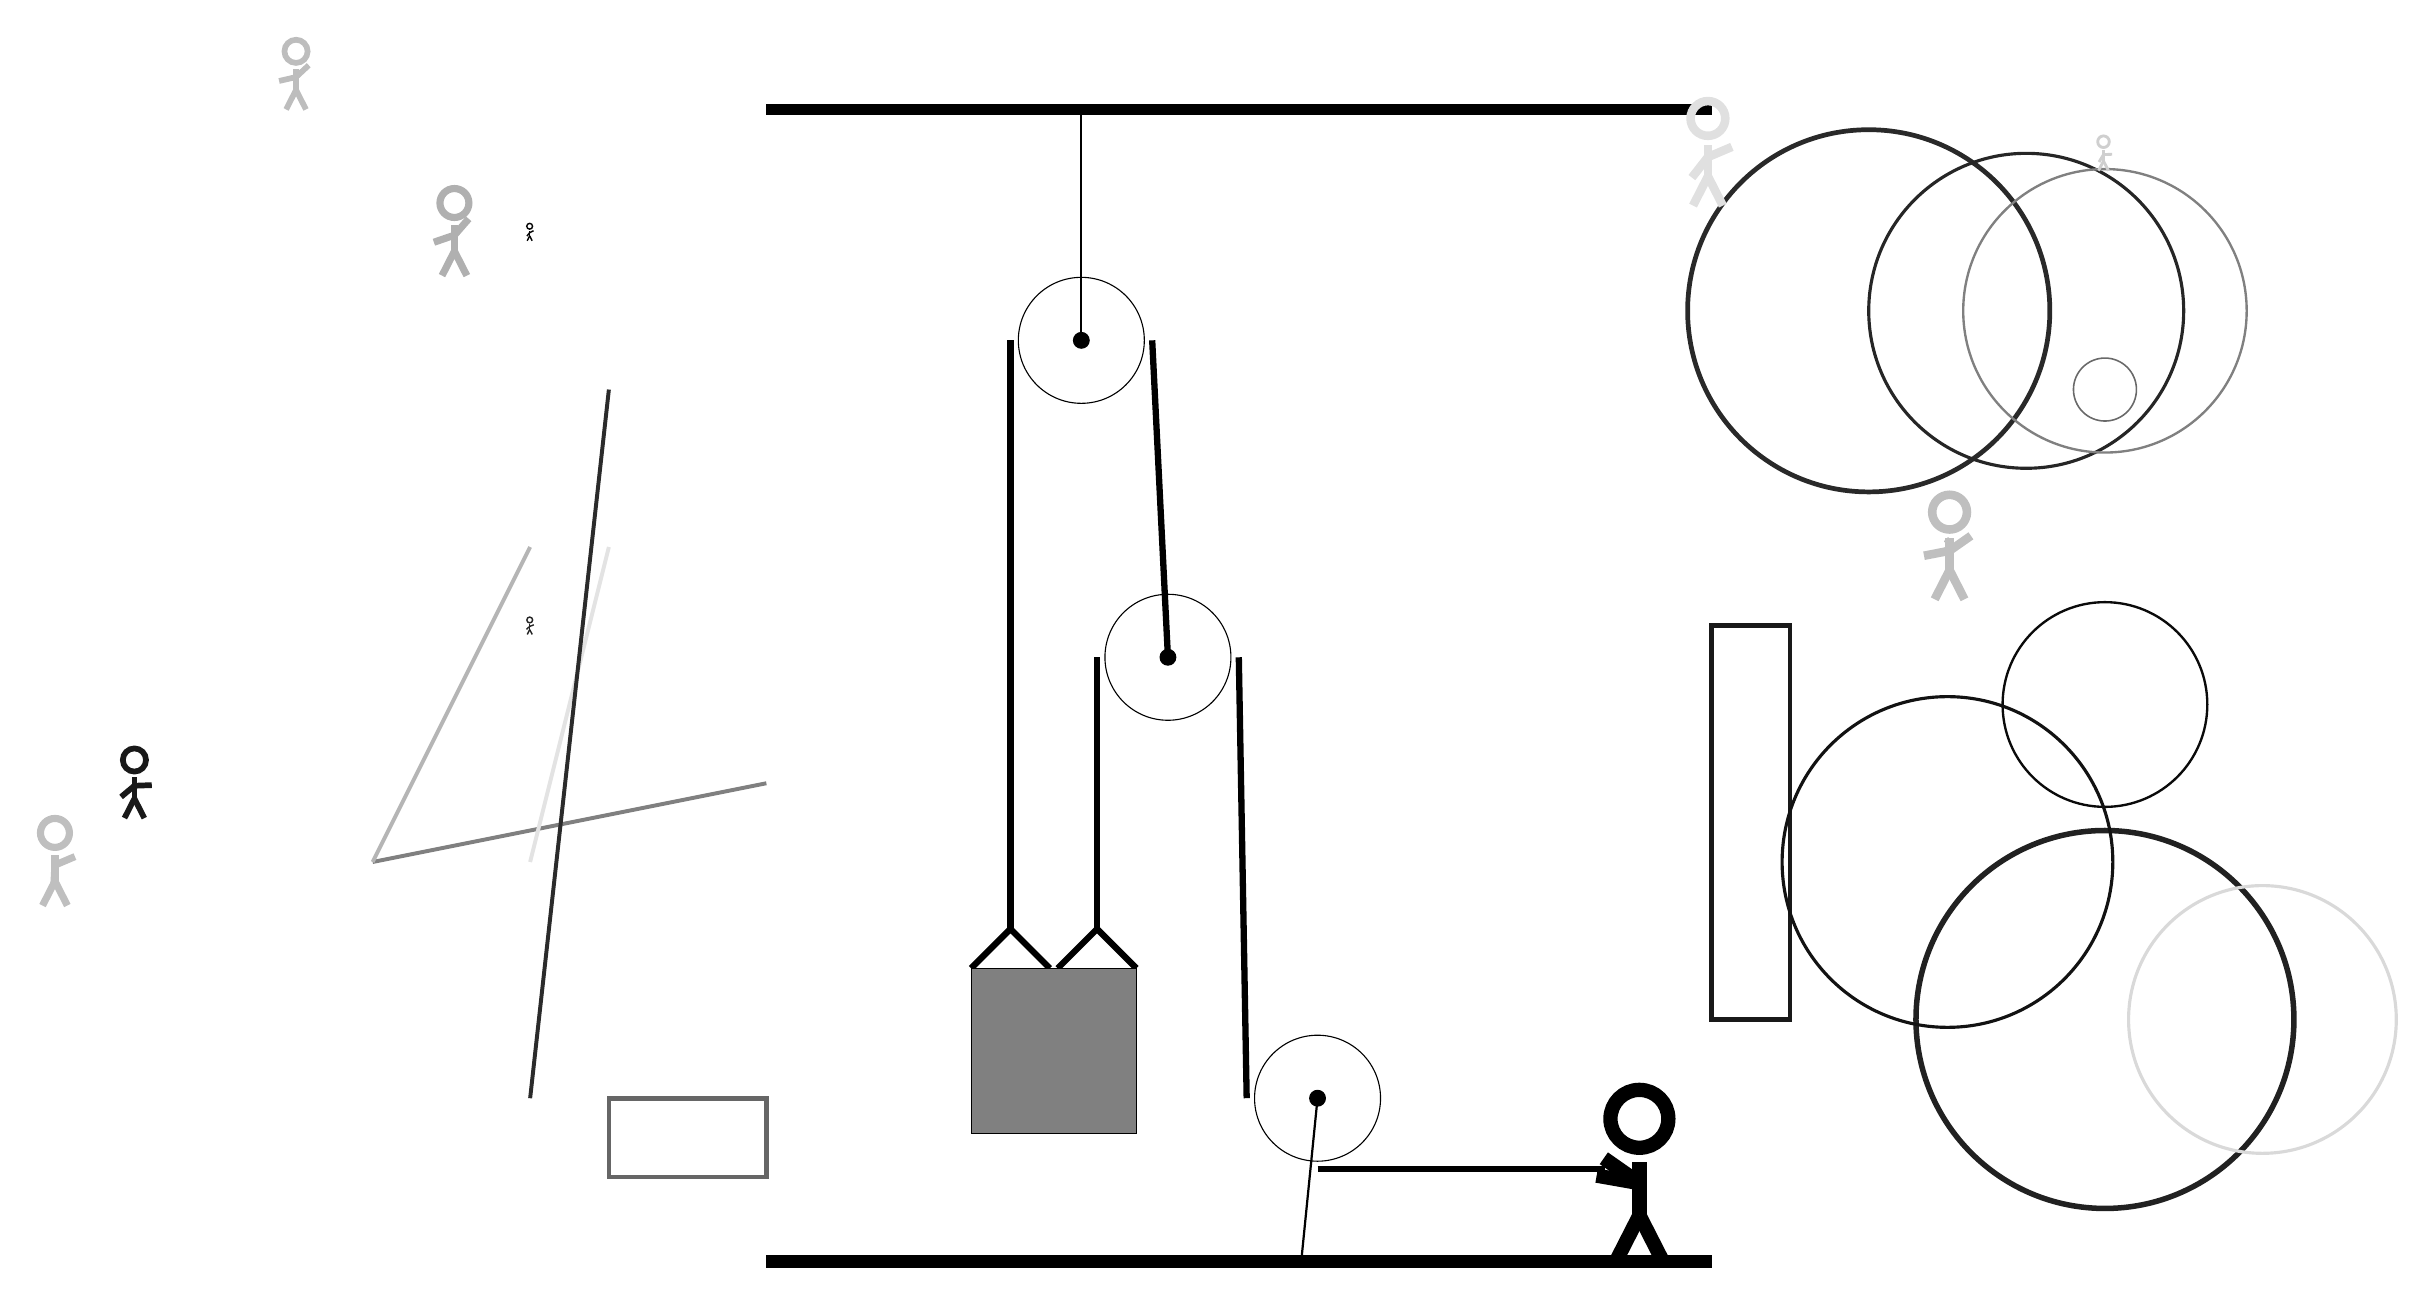
\begin{tikzpicture}
			%%%%% START %%%%%
			
			\draw[fill=black] (-2, 11.5) rectangle (10, 11.625);
			
			\draw (2, 8.625) circle (0.8);
			\draw[fill=black] (2, 8.625) circle (0.1);
			\draw[thick] (2, 8.625) -- (2, 11.5);
			
			\draw (3.1, 4.6) circle (0.8);
			\draw[fill=black] (3.1, 4.6) circle (0.1);
			
			\draw (5, -1) circle (0.8);
			\draw[fill=black] (5, -1) circle (0.1);
			\draw[thick] (5, -1) -- (4.8, -3);
			
			\draw[line width = 0.8mm]  (0.6, 0.65) -- (1.1, 1.15) -- (1.6, 0.65);
			\draw[line width = 0.8mm]  (1.7, 0.65) -- (2.2, 1.15) -- (2.7, 0.65);
			\draw[fill=black!50] (0.6, 0.65) rectangle (2.7, -1.45);
			
			\draw[line width = 0.8mm] (1.1, 8.625) -- (1.1, 1.15);
			\centerarc[line width = 0.8mm](2, 8.625)(0:180:0.9);
			\draw[line width = 0.8mm] (2.9, 8.625) -- (3.1, 4.6);
			\draw[line width = 0.8mm] (2.2, 4.6) -- (2.2, 1.15);
			\centerarc[line width = 0.8mm](3.1, 4.6)(0:180:0.9);
			\draw[line width = 0.8mm] (4.0, 4.6) -- (4.1, -1);
			\centerarc[line width = 0.8mm](5, -1)(180:270:0.9);
			\draw[line width = 0.8mm] (5, -1.9) -- (8.65, -1.9);
			
			\node[line width=0.5mm, color=black!25] at (-11, 2) {\Strichmaxerl[5][87][23]};
			
			\node[line width=0.6mm, color=black!90] at (-10, 3) {\Strichmaxerl[4][40][2]};
			\draw [line width=0.6mm, color=black!84](12, 9) circle (2.3);
			\draw[line width=0.6mm, color=black!90] (10, 0) rectangle (11, 5);
			\node[line width=0.6mm, color=black!55] at (13, 6) {\Strichmaxerl[1][13][60]};
			\draw [line width=0.7mm, color=black!87](15, 0) circle (2.4);
			\draw[line width=0.5mm, color=black!50](-7, 2) -- (-2, 3);
			\node[line width=0.6mm, color=black!25] at (13, 6) {\Strichmaxerl[6][11][35]};
			\draw [line width=0.3mm, color=black!96](15, 4) circle (1.3);
			
			\draw[line width=0.5mm, color=black!29](-5, 6) -- (-7, 2);
			\node[line width=0.7mm, color=black!31] at (-6, 10) {\Strichmaxerl[5][19][49]};
			\draw [line width=0.2mm, color=black!59](15, 8) circle (0.4);
			\node[line width=0.7mm, color=black!12] at (10, 11) {\Strichmaxerl[6][52][23]};
			
			\draw [line width=0.4mm, color=black!93](13, 2) circle (2.1);
			\node[line width=0.5mm, color=black!26] at (-8, 12) {\Strichmaxerl[4][13][43]};
			\draw[line width=0.5mm, color=black!11](-5, 2) -- (-4, 6);
			\draw[line width=0.6mm, color=black!60] (-4, -1) rectangle (-2, -2);
			
			\draw [line width=0.4mm, color=black!85](14, 9) circle (2.0);
			\node[line width=0.3mm, color=black!98] at (-5, 10) {\Strichmaxerl[1][51][27]};
			\draw [line width=0.3mm, color=black!50](15, 9) circle (1.8);
			\draw [line width=0.4mm, color=black!15](17, 0) circle (1.7);
			\node[line width=0.6mm, color=black!19] at (15, 11) {\Strichmaxerl[2][59][2]};
			
			\draw[line width=0.5mm, color=black!83](-5, -1) -- (-4, 8);
			\node[line width=0.6mm, color=black!86] at (-5, 5) {\Strichmaxerl[1][42][21]};
			
			\node at (9, -2) {\Strichmaxerl[10][-35][170]};
			
			\draw[fill=black] (-2, -3) rectangle (10, -3.15);
			
			%%%%% END %%%%%
		\end{tikzpicture}
	\end{figure}	
\end{document}